\documentclass{article}

% if you need to pass options to natbib, use, e.g.:
%     \PassOptionsToPackage{numbers, compress}{natbib}
% before loading neurips_2020

% ready for submission
% \usepackage{neurips_2020}

% to compile a preprint version, e.g., for submission to arXiv, add add the
% [preprint] option:
%     \usepackage[preprint]{neurips_2020}

% to compile a camera-ready version, add the [final] option, e.g.:
%     \usepackage[final]{neurips_2020}

% to avoid loading the natbib package, add option nonatbib:
\usepackage[final]{neurips_2020}
\usepackage[utf8]{inputenc} % allow utf-8 input
\usepackage[T1]{fontenc}    % use 8-bit T1 fonts
\usepackage{hyperref}       % hyperlinks
\usepackage{url}            % simple URL typesetting
\usepackage{booktabs}       % professional-quality tables
\usepackage{amsfonts}       % blackboard math symbols
\usepackage{nicefrac}       % compact symbols for 1/2, etc.
\usepackage{microtype}      % microtypography
\usepackage{graphicx}

\title{Author Name Disambiguation Algorithm}

% The \author macro works with any number of authors. There are two commands
% used to separate the names and addresses of multiple authors: \And and \AND.
%
% Using \And between authors leaves it to LaTeX to determine where to break the
% lines. Using \AND forces a line break at that point. So, if LaTeX puts 3 of 4
% authors names on the first line, and the last on the second line, try using
% \AND instead of \And before the third author name.

\author{%
 ZhiCheng Ji \\
  Tsinghua University\\
  \texttt{jizc19@mails.tsinghua.edu.cn} \\
  % examples of more authors
  \And
  Zaiyuan Lu \\
  % Affiliation \\
  Tsinghua University\\
  \texttt{lzc19@mails.tsinghua.edu.cn}\\
  % \AND
  % Coauthor \\
  % Affiliation \\
  % Address \\
  % \texttt{email} \\
  % \And
  % Coauthor \\
  % Affiliation \\
  % Address \\
  % \texttt{email} \\
  % \And
  % Coauthor \\
  % Affiliation \\
  % Address \\
  % \texttt{email} \\
}

\begin{document}

\maketitle

\section{Introduction}

The growth of scientific literature makes the problem of Name Disambiguation more difficult 
and urgent. Although this subject has been extensively studied in academia and industry, 
the problem has not been solved well due to the clutter of data and the complexity of the same name scenario.
AMiner together with Biendata held a competition during the last months of 2019 aiming for 
new algorithms to tackle this problem. The competition has finished and the winning 
team(Ziyue Quao and Hanxue Wang) achieved a final F1 score of 0,90327. Our new research 
tries to improve the existing method and find more useful information’s to distinguish different authors

\section{Data acquiring}

The data will only be acquired from the Aminer’s “Who is Who” competition data. 
This set of information contains a trainset and a validation set with a substantial size. 

\section{Work planning}

\begin{itemize}
     \item 6-8 weeks
     
     learn the algorithm used in the competition

     \item 9-10 weeks
     
     try the model in the competition
     
     \item 11-15 weeks
     
     improve the model

\end{itemize}

\section{Algorithms used}

There are several indications to distinguish whether a paper belongs to a certain author. 
One of which is reviewing coauthors. If a paper is written by author A and B, and another 
paper is also written by the authors the same name, then it is very likely that the authors
 A and B has written these papers. Besides coauthoring, another feature would be the specific 
 research organization the author is in. These are rules based matching techniques. Then, 
 a clustering analysis will be conducted using DBSCAN


\section{Testing}

We plan to use the evaluation method of the competition based on the Macro Pairwise-F1.

\begin{figure}
     \centering
     % \fbox{\rule[-.5cm]{0cm}{4cm} \rule[-.5cm]{4cm}{0cm}}
     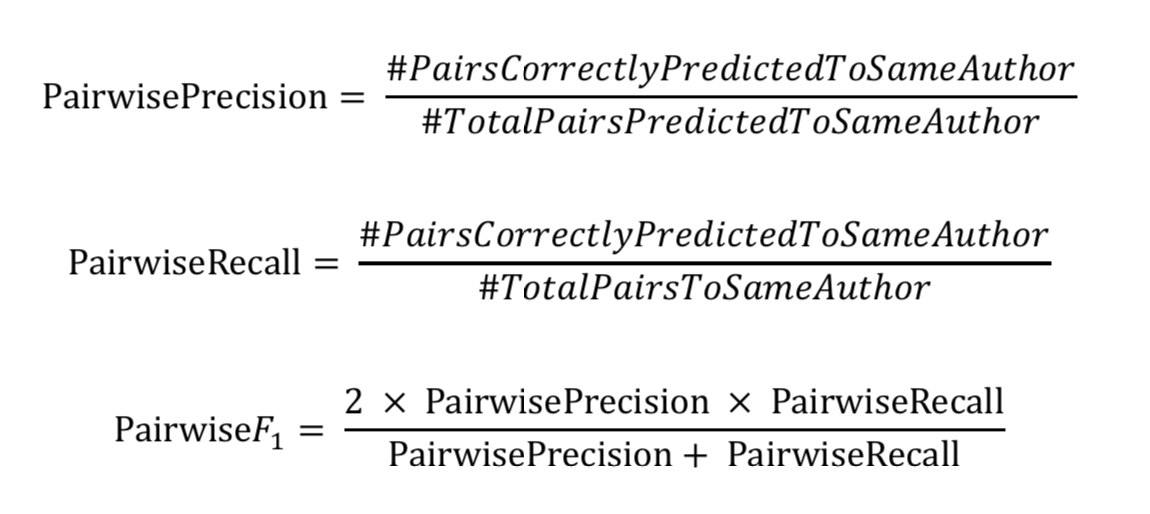
\includegraphics[scale=0.5]{31568965826.png}
     \caption{Evaluation Method}
\end{figure}

\end{document}